\chapter{Répartition des sources de production d'énergies}
% \section{}
% \section{Réutilisation des sources de chaleur}

L'emplacement des points de production sont importants dans la lutte contre le gaspillage énergétique.
Plusieurs points importants entrent en ligne de compte, le coût du transport de cette énergie ainsi que les pertes liée à ce mode de transport.
Peu importe la technologie utilisée, les lois de la thermodynamique rendent impossible le transport d'énergie gratuit.

\section{Perte d'énergie en chaleur}

Prenant en compte la 1ère loi de la thermodynamique, lors de toute transformation, il y a
conservation de l'énergie.
Ainsi, dans un espace clos, l'énergie ne peut varier.
Prenons pour espace le câble qui fait transiter l'énergie de la production à la consommation.

Le transport de l'énergie va transformer en chaleur une partie de celle-ci en raison
des forces de frottement des électrons sur les atomes.

Il est possible de réduire cette perte en utilisant des matériaux plus conducteurs que
d'autres, mais il n'est pas possible de l'annuler.
De plus, pour des raisons économiques, ces matériaux supraconducteurs ne peuvent être
déployés en masse du fait de leur coût, et des conditions nécessaires à leur stabilité.
Le Diborure de magnésium $MgB_2$ est un des matériaux ayant la plus haute température
critique avec 39 K (-234 C).

Aujourd'hui, la majorité des câbles électriques mondiaux sont en cuivre ou en aluminium,
on va s'intéresser plus particulièrement au cuivre qui possède le meilleur rendement.

Pour calculer la perte d'énergie dans un câble en cuivre, on peut utiliser
la formule $Loss = I^2\times R$ avec $I$ pour l'intensité, exprimée en ampère, et $R$ en Ohm.

On peut exprimer les Ohms avec la formule suivante : $R = \frac{V}{I_r}$
avec $V$ pour le voltage et $I_r$ pour l'intensité perdu par la résistance du matériaux.

Cette formule montre que augmenter l'intensité augmente beaucoup plus la perte d'énergie
que le voltage.

Cette relation explique pourquoi il est plus rentable de créer des lignes a haute tension
pour de longues distances.
Cependant, un voltage élevé amène d'autres problèmes comme un électromagnétisme intense,
c'est pourquoi les lignes à haute tensions sont en haut de grand pilonnes.

C'est RTE en France qui à décide du voltage et fait ce choix pour minimiser les coût de
fabrication et le coût de la perte de l'exploitation des lignes.

En comparaison, les lignes électriques du Canada ou des États-Unis utilisent un voltage
plus important car les distances que parcours l'énergie est plus importante.

En France, on utilise la norme \texttt{NF\_C18-510} pour classer les lignes électriques


\begin{center}
  \begin{table}[h]
    \begin{tabular}{|l|l|l|}
      Tension    & Courent Alternatif     & Courent Continue \\
      Très basse & $U_n \leq 50V$         & <COMPLETE>       \\
      Basse      & $50V < U_n \leq 1kV$   & <COMPLETE>       \\
      Haute      & $1kV < U_n \leq 50kV$  & <COMPLETE>       \\
      Très Haute & $U_n > 50kV$           & <COMPLETE>       \\
    \end{tabular}
  \end{table}
\end{center}

Chacune de ces tensions sont utilisé pour des besoins spécifiques.

Le courent alternatif est plus utilisé car chauffant moins

\section{Topologie et répartition}

Les méthodes de production et de distributions d'énergies sont en train de changer en réponse
à la diversification des moyen de production.

Avec des consommateur pouvant générer de l'électricité sur leurs toits, ou dans leurs jardin,
ceux-ci deviennent ce que l'on appèle en anglais des \textit{prosumer} pour producer (producteur)
consumer (consommateur).

De le futur de la distribution, tout les nœuds du réseau serons susceptible de produire de l'énergie,
cette distribution deviens bi-directionnel.

De nombreux défi existent pour concevoir cette transformation, nombreux sont ceux traité en amont de ce papier,
cependant il reste un problème de taille pour finir ce thème.

Comment mettre a jours un réseau existant à bas voltage pour faciliter la mise en œuvre des technologies
de smart grid ?

Pour ce faire, la topologie est un outil mathématique adéquat pour répondre a ces problématiques d'optimisation
et de partage de l'information avec ces nœuds.
La disposition des \textit{prosumer} sera les nœuds d'un graphe avec les lignes électrique des liens du graphe.

La première remarque du système actuel est que la distribution d'énergie contribue de 8 à 15\% de perte
d'énergie en chaleur.

La topologie traditionnel des réseau de distribution est en forme d'arbre.
Dans le schema \ref{fig:ieee_radial_tree}, le symbole du nœud 799 est un transformateur qui
fonctionne en tant qu'interrupteur on/off tandis que le symbole entre les nœuds
709 et 775 est un transformateur qui contrôle le voltage.

\begin{SCfigure}[2][h]
  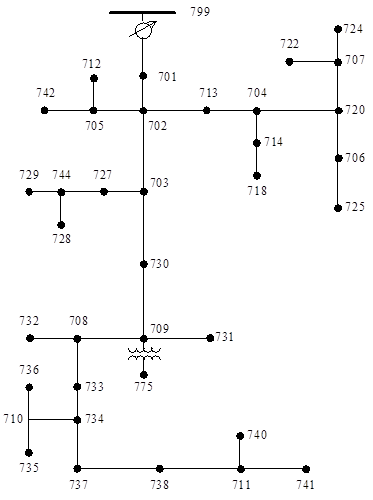
\includegraphics[scale=0.5]{media/ieee_radial_tree.png}
  \caption{
      IEEE 37 nœud de test\newline
      \tiny{Source:\newline
        Smart Grid Topology Designs
      }
  }
  \label{fig:ieee_radial_tree}
\end{SCfigure}

Considérons un réseau de distribution d'électricité basse tension existant dans une zone urbaine modélisée,
$G = (N, A)$ pour un ensemble de $n$ positions $N = \lbrace 1 \dots, n \rbrace$ de sorte que la topologie soit un arbre enraciné
au nœud $n_0$.

Historiquement, l'électricité devait être fournie par le contrôleur en réponse à la demande des consommateurs,
de sorte que les graphiques étaient considérés comme orientés.
Nous faisons quelques hypothèses simplificatrices pour traiter le flux de courant alternatif non linéaire.

Considérons que l'ensemble $N \backslash n_0$ est divisé en ensembles $C$ des utilisateurs finaux qui restent des consommateurs et
en ensemble $P$ des nouveaux \textit{prosumer}.

L'électricité peut être renvoyée par le \textit{prosumer} dans le réseau de distribution sans qu'il soit nécessaire
de créer des arêtes supplémentaires, et elle peut être contrôlée et surveillée par des dispositifs de commutation.
On peut donc supposer que le réseau existant est modélisé par $\bar{G} = (N, E)$

Considérant une horizon temporelle $T$,
tous les utilisateurs $i \in N \backslash n_0$ consomment un quantité
$EC^t_i$ d'énergie à un temps $t$.
Tous les \textit{prosumer} $i \in P$ génèrent une quantité
$EG^t_i$ d'énergie à un temps $t$.

À chaque unité de temps $t$ l'énergie demandé est de $Q^t_i$ pour chaque consommateurs
$i \in C$ tel que $Q^t_i = -EC^t_i$.

À chaque unité de temps $t$ l'énergie demandé est de $Q^t_i$ pour chaque \textit{prosumer}
$i \in P$ tel que $Q^t_i = EG^T_i - EC^t_i$.

Si $Q^t_i = 0$, alors le \textit{prosumer} est auto-suffisant, il ne nécessite
ni d'export d'énergie, ni d'import.
Si $Q^t_i > 0$, alors le \textit{prosumer} a un excès d'énergie, il devra en vendre.
Si $Q^t_i < 0$, alors le \textit{prosumer} a un déficit d'énergie, il devra en acheter.

Assumant le réseau comment communautaire, et que le nœud $n_0$ produit de l'énergie
$\sum_{i \in N \backslash \lbrace n_0 \rbrace} Q^t_i < 0$ et reçois de l'énergie
$\sum_{i \in N \backslash \lbrace n_0 \rbrace} Q^t_i > 0$.

Donnons
$Q^t_{n_0} = \sum_{i \in N \backslash \lbrace n_0 \rbrace} Q^t_i$
et
$\bar{Q} = \max_{t \in T} \sum_{i \in N \backslash \lbrace n_0 \rbrace} \lvert Q^t_i \rvert$
qui doivent être l'électricité maximum que doit transporter toute connexion.

On prend en compte la perte d'énergie en tant que "Loss factor" $L \in \lbrack 8, 15 \rbrack \%$

La topologie des variables $x_{ij}$ indiquent l'arc $(i, j)$ sélectionné.
Le flow $y^t_{ij}$ indique la quantité d'énergie transporté entre $i$ et $j$ pour un temps $t$.

La constante $a_{ij}$ prendre la valeur 1 si l'arc $(i,j) \in E$ signifiant qu'il est stable et
fait partit du réseau de distribution, et prend la valuer 0, si l'arc $(,j) \notin E$, signifiant
qu'il ne fait pas partit du réseau.

La formule deviens

\begin{equation} \label{prosumer_1}
  Eq = \min \sum_{(i, j) \in A} c_{ij} x_{ij} + \sum_{t \in T} \sum_{(i,j) \in A} y^t_{ij}
\end{equation}

Sujet à

\begin{equation} \label{prosumer_2}
  \sum_{i \in N} (a_{ij} + x_{ij}) \ge 1
\end{equation}
\begin{equation} \label{prosumer_3}
  \sum_{i \in N} (a_{ij} + x_{ij}) \ge 1
\end{equation}
\begin{equation} \label{prosumer_4}
  \sum_{i \in N} (a_{ij} + x_{ij}) \ge 1
\end{equation}
\begin{equation} \label{prosumer_5}
  \sum_{i \in N} y^t_{ij} + (1 + L) Q^t_j = \sum_{i \in N} y^t_{ij}
\end{equation}
\begin{equation} \label{prosumer_6}
  y^t_{ij} \le \bar{Q}(a_{ij} + x_{ij})
\end{equation}
\begin{equation} \label{prosumer_7}
  a_{ij} + x_{ij} + a_{ji} + x_{ji} \le 1
\end{equation}
\begin{equation} \label{prosumer_8}
  x_{ij} \in \lbrace 0, 1 \rbrace
\end{equation}
\begin{equation} \label{prosumer_9}
  y^t_{ij} \ge 0
\end{equation}

Donnons $c_{ij}$ le coût d'installation d'un nouvel arc $ij \in A$ dans
le réseau amélioré.

% 1
$Eq$ est la fonction objectif \ref{prosumer_1} qui minimise le coût d'ajout de nouveau arc
ainsi que la perte d'énergie.
% 2
L'inégalité \ref{prosumer_2} s'assure que chaque consommateur reste connecté au réseau principale.
% 3 et 4
Les inégalités \ref{prosumer_3} et \ref{prosumer_4} s'assurent que chaque \textit{prosumer} reste connecté au réseau principale.
Vu que chaque \textit{prosumer} a la capacité de recevoir et de donner de l'énergie, la vérification
est fait en duplex.
% 5
L'égalité \ref{prosumer_5} est une contrainte de conservation de l'énergie en prenant en compte la perte d'énergie $L$.
% 6
L'inégalité \ref{prosumer_6} est le lien des variables et limite la quantité d'énergie par lien.
% 7
L'inégalité \ref{prosumer_7} interdit la création d'un lien si il en existe déjà un.
% 8 et 9
Les contraintes \ref{prosumer_8} et \ref{prosumer_9} définissent le domaine des variables.

Ces formules nous donne pour 25\% de \textit{prosumer}, et une perte de 8\% le schema \ref{fig:ieee_radial_tree_optimized}

\begin{SCfigure}[2][h]
  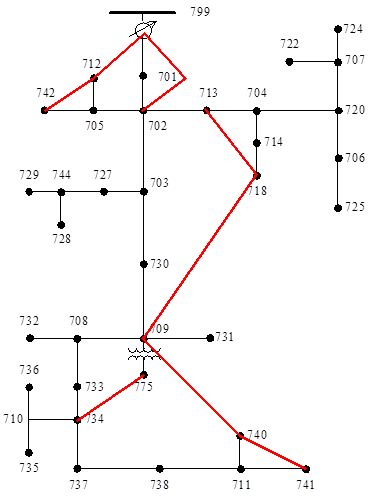
\includegraphics[scale=0.5]{media/ieee_radial_tree_optimized.png}
  \caption{
      IEEE 37 nœud de test optimisé pour des prosumer\newline
      \tiny{Source:\newline
        Smart Grid Topology Designs
      }
  }
  \label{fig:ieee_radial_tree_optimized}
\end{SCfigure}

Cette topologie apporte des réductions de pannes, du trajet de l'énergie et donc de ses pertes énergétique, pour un coût
pensé minimal.

Les données des calcules sont disponible sur le papier Smart Grid Topology Designs de Paula Carroll et Cristina Requejo